\documentclass[titlepage,oneside,a4paper,11pt]{book} % version électronique
%\documentclass[titlepage,twoside,letterpaper,openright,12pt]{book} % version imprimée

%-----------------PDFLATEX----------------------
% Pour pdflatex, décommenter les lignes qui suivent
%\usepackage[latin1]{inputenc} % encodage des caractères. choix: utf8, latin1, applemac
%\usepackage[T1]{fontenc}
\usepackage[utf8]{inputenc} % encodage des caractères. choix: utf8, latin1, applemac
%\usepackage[T1]{fontenc}


% choix du style de police (tout commenter pour les polices TeX habituelles [computer modern])
\usepackage[table,xcdraw]{xcolor}
\usepackage{mathpazo} % utilise Palatino pour les mathématiques (mettre en premier)
\usepackage{tgpagella} % utilis
\usepackage{amsfonts}		% ajoute des polices mathématique
\usepackage{amsmath}        % ajoute des environnements mathématiques
\usepackage{float}
\usepackage{fancyhdr}
\pagestyle{plain}
\usepackage{bm}				% ajoute des caractères grecs en gras
\usepackage{wrapfig}
\usepackage{mathrsfs}		% ajoute une meilleure police calligraphique pour certains symboles
\usepackage{setspace} 		% gère l'interligne
\usepackage[french]{babel}  % comment this line if the thesis is in English
%\usepackage[babel=true,kerning=french,protrusion=true,expansion=auto,spacing,tracking]{microtype}
\usepackage{graphicx}		% gère l'insertion des figures
\usepackage{subfig}			% permet d'ajouter des sous-figures
\usepackage{geometry}		% gère les dimensions du document (mise en page)
\usepackage{hyperref}
\hypersetup{
    colorlinks=true,
    linkcolor=blue,
    filecolor=magenta,      
    urlcolor=cyan,
    pdftitle={Overleaf Example},
    pdfpagemode=FullScreen,
    }
\usepackage[export]{adjustbox}
% \geometry{
 %a4paper,
 %total={170mm,257mm},
 %left=20mm,
 %top=20mm,
 %}
%\usepackage[x11names,svgnames]{xcolor}
\usepackage{fancybox}		% définit des macros pour des boîtes, des cadres, etc.
\usepackage{url}            % permet de typographier des url
\usepackage{comment}
\setlength{\parindent}{0pt}


%\input {macros.tex}

\begin{document}

{Électricité et Magnétisme}
\hfill
{203-NYB 102} \\ 
{Chargé de Cours: Samuel Houle}
\hfill
{Hiver 2024}\\
\begin{center}
\textbf{Circuits et Courant Alternatif}
\end{center}

Un circuit AC est une combinaison d'éléments de circuit et d'une source qui produit une tension alternative.  Cette tension (qui dépend du temps) est décrite par
\begin{equation}
V_{ac}(t) = V(t) = V_{\mathrm{max}}\sin{(\omega t+\varphi)}
\label{eq:alt}
\end{equation}
%\begin{comment}
\begin{wrapfigure}{r}{0.4\textwidth}
  \begin{center}
    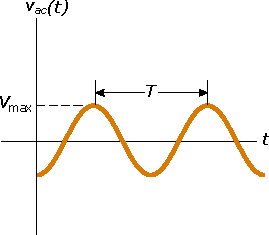
\includegraphics[width=0.4\textwidth]{v_output.pdf}
    \caption{Tension en fonction du temps à la sortie d'une source de tension alternative.}
    \label{fig:ac}
  \end{center}
\end{wrapfigure}
%\end{comment}
où $V_{\mathrm{max}}$ est la valeur maximale de tension que peut produire la source AC. On nomme aussi $V_{\mathrm{max}}$ \textbf{l'amplitude} de la tension. Comme pour tout mouvement d'oscillation (un mouvement qui peut être décrit par une fonction sinusoïdale), la tension possède une fréquence angulaire $\omega$, une fréquence $f$ et une période $T$.  Ces quantités sont reliées de la façon suivante
\begin{equation*}
\omega = 2\pi f = \frac{2\pi}{T}
\end{equation*}
C'est la fréquence de la source qui détermine la fréquence du courant que celle-ci générera dans un circuit. La forme d'une tension a lternative sinusoïdale est illustrée à la Figure \ref{fig:ac}.\\

\textbf{Éléments résistifs dans un circuit AC}\\

Commençons par considérer le circuit AC le plus simple, celui d'une résistance branché à une source AC 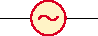
\includegraphics[height=3ex,valign=M]{source_symbol.pdf}. En l'absence de champ magnétique circulant au travers de la boucle,  la somme des tensions aux bornes du circuit doit être nulle en tout temps (loi de Kirchhoff), ce qui mène à
\begin{equation*}
V_{ac}(t) + V_R(t) = 0 
\end{equation*}
La norme de la tension aux bornes de l'élément résistif est égal à la tension de la source
\begin{equation*}
V(t) \equiv V_R(t) = V_{\mathrm{max}} \times \sin (\omega t+\varphi)
\end{equation*}
où $V_R(t)$ est la \textbf{tension instantanée} aux bornes de la résistance.  Dans ce cas, la loi d'Ohm impose que
\begin{equation}
I_R(t) = \frac{V_R(t)}{R} = \frac{V_{\mathrm{max}}\times \sin (\omega t+\varphi)}{R} = I_{\mathrm{max}}\times\sin (\omega t + \varphi)
\end{equation}
avec $I_{\mathrm{max}}=V_{\mathrm{max}}/R$. Nous pouvons voir clairement que les \textbf{phases} de la tension et du courant sont \textbf{identiques} et sont égales à $\omega t+\varphi$.  Mis à part leur amplitude, le courant et la tension varient de façon identique dans le temps.  On dit alors qu'ils sont en phase \footnote{La phase est de loin la notion la plus importante pour décrire l'interaction de différentes quantités oscillantes. Plus précisément la \emph{différence} de phase. La phase \emph{absolue} n'a aucune importance.  Toute la physique de l'interférence émerge de cette notion. Rappelez-vous les \href{https://en.wikipedia.org/wiki/Double-slit_experiment}{fentes de Young}, où l'amplitude lumineuse s'annulait pour certaines positions bien précises. Si deux signaux qui interfèrent possède la même amplitude, il peut y avoir une interférence totale (signal résultant nul) et si ces deux amplitudes diffèrent, il y aura alors interférence partielle.}.\\

\begin{wrapfigure}{r}{0.5\textwidth}
  \begin{center}
    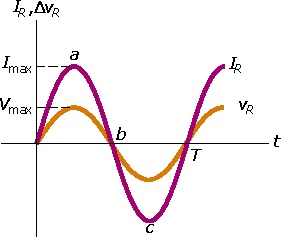
\includegraphics[width=0.4\textwidth]{v_i_R.pdf}
    \caption{Représentation temporelle du courant $I_R$ et de la tension $V_R$.  Les deux quantités sont en phase, ce qui signifie que leurs maxima et leur minima correspondent aux mêmes instants.}
    \label{fig:i_v_R_time}
  \end{center}
\end{wrapfigure}

Pour les éléments résistifs, il n'y a pas de nouvelle physique en ce qui concerne le lien entre le courant et la tension.  Le courant dans une résistance est toujours en phase avec la tension et se comporte comme dans un circuit à courant continu, tel qu'illustré à la Figure \ref{fig:i_v_R_time}.\\


Une autre manière d'illustrer le lien entre le courant et la tension est d'utiliser un \textbf{phaseur}. Un phaseur n'est rien d'autre qu'un vecteur possédant une longueur finie et qui tourne de manière anti-horaire à la fréquence angulaire associée à la quantité qu'il représente.  C'est une représentation mathématique particulièrement utile lorsque vient le temps d'analyser des signaux qui n'ont pas nécessairement la même phase. Le diagramme des phaseurs pour la tension et le courant dans un circuit résistif est illustré à la Figure \ref{fig:i_v_R_phaseur}.\\ 

Dans le cas d'un circuit purement résistif, comme le courant et la tension sont en phase, l'orientation de leurs phaseurs respectifs sera toujours alignée dans la même direction. Seule les longueurs de ceux-ci resteront constantes.
La projection des phaseurs sur l'axe vertical correspond à ce qui est illustré à la Figure \ref{fig:i_v_R_time}. Nous pouvons donc nous servir des projections d'un phaseur pour obtenir la représentation les valeurs de courant et de tension qui varient de manière sinusoïdale en fonction du temps. L'avantage de l'approche par phaseurs est que la relation de phase devient évidente.\\


Pour un circuit résistif, la valeur moyenne du courant sur une période est de zéro. Le courant passe autant de temps dans les négatifs que dans les positifs (ce qui correspond à un courant allant dans un sens ou dans l'autre). Toutefois, la direction du courant n'a pas d'importance sur le caractère résistif du circuit.  La résistance transforme l'énergie cinétique des électrons en énergie thermique. L'énergie cinétique étant proportionelle à $v^2$, le signe $\pm$ devant $v$ n'a pas d'importance sur la quantité totale d'énergie qui sera dissipée au travers de la résistance.  La puissance dissipée dans une résistance est donnée par
\begin{wrapfigure}{l}{0.4\textwidth}
  \begin{center}
    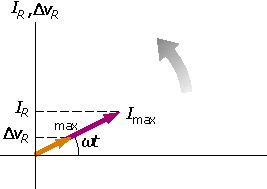
\includegraphics[width=0.4\textwidth]{v_i_R_phaseur.pdf}
    \caption{Représentation sous forme de phaseurs pour un circuit purement résistif La longueur des vecteurs (leur valeur maximale) ne change jamais, mais leur orientation, elle, dépend du temps.}
    \label{fig:i_v_R_phaseur}
  \end{center}
\end{wrapfigure}
\begin{align*}
    P&=I^2R\\
    P&=I_{\mathrm{max}}^2\sin^2\omega t\times R
\end{align*}

Ici, la quantité d'intérêt n'est pas la puissance maximale dissipée en un instant bien précis mais plutôt la puissance dissipée de façon moyenne.  On nomme cette puissance moyenne la puissance \textbf{rms} (\emph{root mean squared}) et elle correspond à la puissance dissipée par le courant \textbf{rms} dans le circuit. On écrit alors

\begin{align*}
    P_{\mathrm{rms}}&=I_{\mathrm{rms}}^2\times R\\
    P_{\mathrm{rms}}&=\Bigg{(}\frac{I_{max}}{\sqrt{2}}\Bigg{)}^2\times R
\end{align*}

Ce résultat vient du fait que le courant moyen, dans le cas d'un courant oscillant de façon sinusoïdale, est donné par sa moyenne temporelle sur une période. Le courant varie comme $I=I_{max}\sin \omega t$ et donc, $I^2 = I^2_{max}\times\sin^2 \omega t$. Ainsi, on peut calculer la valeur moyenne de $I^2$ en calculant la valeur moyenne de $\sin^2 \omega t$.  Un graphique de $\cos^2 \omega t$ en fonction du temps est identique à celui pour $\sin^2 \omega t$ hormis le fait que les points sont décalés d'une phase $\pi/2$. Ainsi, on sait que, sur une période $\langle sin^2 \omega t \rangle = \langle cos^2 \omega t \rangle$\footnote{Nous utilisons ici la notation $\langle . \rangle$ pour dénoter la moyenne temporelle.}. En combinant cela avec l'identité trigonométrique bien connue voulant que $\cos^2 \theta + \sin^2 \theta =1$, nous obtenons
\begin{align*}
    \langle \sin^2 \omega t\rangle + \langle \cos^2 \omega t\rangle = 2\langle \sin^2\omega t\rangle &=1\\
    \langle \sin^2\omega t\rangle &= \frac{1}{2}
\end{align*}
En substituant ce résultat dans l'expression pour $I^2$, nous obtenons que
\begin{align*}
    I^2_{\mathrm{rms}} &= \langle I^2 \rangle = \frac{I_{max} ^2}{2}\\ 
    I_{\mathrm{rms}}  &= \frac{I_{max}}{\sqrt{2}} \\
\end{align*}
ce résultat est illustré à la Figure \ref{fig:rms}.
\begin{figure}[H]
\centering
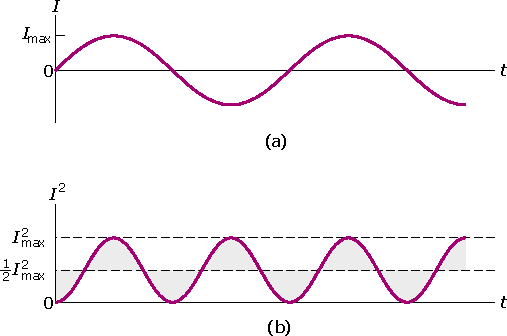
\includegraphics[width=.8\textwidth]{rms.pdf}
\caption{(a) Graphique du courant alternatif traversant une résistance en fonction du temps. (b) Graphique du courant traversant une résistance en fonction du temps mis au carré. Les régions en gris au-dessus et au-dessous de la droit pointillée $I^2_{max}/2$ ont la même surface. La valeur moyenne de $I^2$ est donc $I_{max}^2/2$.}
\label{fig:rms}
\end{figure}
d'où l'expression obtenue pour la puissance rms dissipée dans un circuit\footnote{Le facteur rms trouvé ici n'est valable que pour un signal sinusoïdal, il serait différent pour des ondes carrées ou encore tout autre type d'onde périodique}. \textbf{La puissance rms correspond à la puissance qui serait dissipée par un courant continu équivalent au courant alternatif, $I_{\mathrm{rms}}$.} Il est aussi pratique courante de discuter de la tension alternative sous sa forme rms
\begin{equation*}
V_{\mathrm{rms}} = \frac{V_{\mathrm{max}}}{\sqrt{2}} = .707 \times V_{\mathrm{max}}    
\end{equation*}

Encore une fois, \textbf{la tension rms correspond à la tension qui causerait une dissipation par une tension continue équivalente à celle de la tension alternative, $V_{\mathrm{rms}}$.} Par exemple, au Québec, lorsqu'on parle d'une tension de 120 V dans les prises murales, on fait référence à la valeur rms de la tension. Ainsi, la valeur $V_{\mathrm{max}}$ qui serait mesurée à l'oscilloscope serait de 170 V. Toutefois, un voltmètre en mode continu indiquerait 120 V.\\

{\Large \textbf{Inductance et circuits à courant alternatif}}\\

L’inductance est une grandeur physique qui mesure la capacité d’un circuit électrique à stocker de l’énergie magnétique. Elle est mesurée en Henry (H) et est définie comme le quotient du flux magnétique créé par un courant traversant un circuit par l’intensité de ce courant.\\

\begin{wrapfigure}{r}{0.5\textwidth}
  \begin{center}
    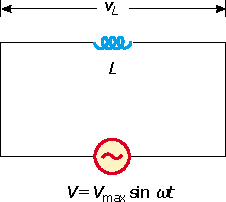
\includegraphics[width=0.4\textwidth]{inductance.pdf}
    \caption{Schéma représentant une inductance en série avec une source de tension.}
    \label{fig:L_circuit}
  \end{center}
\end{wrapfigure}

La tension aux bornes d’une inductance est proportionnelle à la dérivée du courant la traversant, selon la loi d’induction de \textsc{Faraday}. Mathématiquement, cela peut être exprimé comme suit:
\begin{equation*}
    V_L(t)=L\frac{dI}{dt}
\end{equation*}

où $V_L(t)$ est la tension aux bornes de l’inductance, $L$ est l’inductance en Henry, et $I$ est le courant traversant l’inductance en ampères.\\

Cette relation montre que la tension aux bornes d’une inductance est directement proportionnelle à la dérivée du courant la traversant. Cela signifie que plus le courant varie rapidement, plus la tension aux bornes de l’inductance sera élevée.\\ %Cette propriété est souvent utilisée dans la conception de circuits électriques pour filtrer les signaux à haute fréquence 1.

Passons maintenant au cas où le circuit est composé simplement d'une source de tension alternative et d'une inductance de valeur $L$. Notons $V_L$, la chute de potentiel aux bornes de l'inductance définie de la façon habituelle $V_L = -L\times dI/dt$. Ainsi, 
\begin{equation*}
    V(t) -L\frac{\mathrm{d}I}{\mathrm{d}t} = 0
\end{equation*}

Remplaçons $V(t)$ par sa forme explicite
\begin{equation}
    V(t) = V_{\mathrm{max}}\sin \omega t =L\frac{\mathrm{d}I}{\mathrm{d}t}
    \label{eq:L_voltage}
\end{equation}
Nous obtenons alors
\begin{align*}
    \mathrm{d}I &= \frac{V_{\mathrm{max}}}{L} \sin \omega t \;\mathrm{d}t\\
    I_L(t) &= \frac{V_{\mathrm{max}}}{L}\int \sin \omega t\; \mathrm{d}t = -\frac{V_{\mathrm{max}}}{\omega L}\cos \omega t
\end{align*}
avec $I_L(t)$ le courant qui traverse l'inductance en fonction du temps. Ainsi,
\begin{equation}
    I_L(t) = \frac{V_{\mathrm{max}}}{\omega L} \sin \Bigg{(}\omega t - \frac{\pi}{2}\Bigg{)}
    \label{eq:i_ind}
\end{equation}

\textbf{Pour une tension d'excitation sinusoïdale, le courant dans une inductance est toujours \emph{hors} phase, étant en retard d'une phase $\pi/2$.} Ce résultat est illustré à la Figure \ref{fig:ind_phaseurs}. \\ 

\begin{figure}[H]
\centering
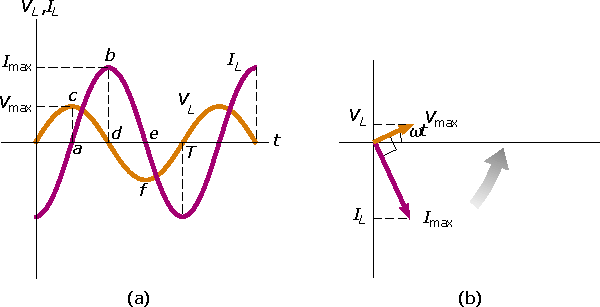
\includegraphics[width=.8\textwidth]{v_i_L_phaseur.pdf}
\caption{(a) Tracés des courants $I_L$ et des tensions $V_L$ instantanés aux bornes d'une inductance. Le courant est déphasé de $-\pi/2$. Au point \emph{a}, le courant est nul alors que la tension au même instant, en \emph{c} est maximale. Aux points \emph{b} et \emph{d}, le courant est maximal pour une tension nulle alors qu'en \emph{e} et \emph{f}, le courant est nul pour une tension minimale. (b) Représentation sous forme de phaseurs pour un circuit inductif.}
\label{fig:ind_phaseurs}
\end{figure}


L'Eq. (\ref{eq:i_ind}) nous renseigne sur le fait que, pour une inductance, le courant maximal est donné par $I_{\mathrm{max}}=V_{\mathrm{max}}/\omega L$. C'est un résultat profond de sens.  Le milieu (dans ce cas la bobine) discrimine entre les différents signaux qui peuvent s'y propager sur une base \emph{fréquentielle}.  Ce n'était pas le cas pour une simple résistance. Le terme $\omega L$ possède bien comme unités des Ohms. La bobine se comporte comme une espèce de résistance dont la valeur change en fonction de la fréquence du signal d'entrée.\\

Définissons la \textbf{réactance} de l'inductance comme
\begin{equation}
    X_L \equiv \omega L
    \label{eq:reac_L}
\end{equation}

La réactance d'un élément de circuit se comporte, du moins au niveau du traitement mathématique du circuit, comme une résistance. Toutefois, la réactance est associée à un élément de circuit qui déphasage le courant de la tension.  C'est pourquoi la réactance d'une simple résistance est nulle. Ainsi,
\begin{equation}
    I_{\mathrm{max}} = \frac{V_{\mathrm{max}}}{X_L}
    \label{eq:L_IV}
\end{equation}

Ainsi, en combinant les Eq. (\ref{eq:L_voltage}) et (\ref{eq:L_IV}), nous obtenons
\begin{align}
    V_L(t) &= -L\times\frac{dI}{dt} = -V_{\mathrm{max}}\times\sin \omega t = -I_{\mathrm{max}}\times X_L\times\sin \omega t \nonumber\\
    V_L(t) &= -I_{\mathrm{max}}\times \omega L\times\sin \omega t 
\end{align}

{\Large \textbf{Condensateurs et circuits à courant alternatif}}\\
\begin{wrapfigure}{r}{0.4\textwidth}
  \begin{center}
    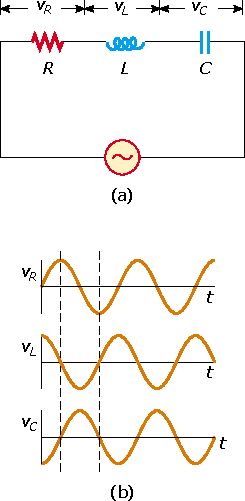
\includegraphics[width=0.4\textwidth]{rlc_schema.pdf}
    \caption{Tension en fonction du temps à la sortie d'une source de tension alternative.}
    \label{fig:rlc_schema}
  \end{center}
\end{wrapfigure}
Le dernier élément de circuit à analyser est le condensateur.  Pour un circuit constitué uniquement d'une source de tension alternative et d'un condensateur en série, nous avons
\begin{equation}
    V_C(t) =\frac{Q(t)}{C}= V_{\mathrm{max}}\times \sin \omega t\\
    \label{eq:c_voltage}
\end{equation}

Ainsi, nous pouvons isoler la charge sur la capacité
\begin{equation*}
    Q(t) = C\times V_{\mathrm{max}}\times \sin \omega t
\end{equation*}
En prenant la dérivée de cette dernière équation, nous obtenons le courant au travers de la capacité
\begin{equation*}
    I_C(t) = \frac{dQ(t)}{dt} = \omega\times C \times V_{\mathrm{max}}\times \cos \omega t
\end{equation*}
Et donc
\begin{equation*}
    I_C(t) = \omega \times C\times V_{\mathrm{max}}\sin \Bigg{(}\omega t + \frac{\pi}{2}\Bigg{)}
\end{equation*}
Encore une fois, le courant est déphasé par rapport à la tension, mais cette fois-ci, le courant est en avance sur cette dernière, son déphasage est positif. Sur un même cycle, le courant atteint son maximum avant la tension. On peut y réfléchir dans les termes suivants.  Lorsque le condensateur est pleinement chargé, il ne peut plus y avoir de charges qui s'y accumulent, le courant est donc nul.  C'est aussi à ce moment que la tension à ses bornes est égale à $V_{\mathrm{max}}$.\\

Ainsi donc,
\begin{equation*}
    I_{\mathrm{max}} = \omega \times C\times V_{\mathrm{max}} = \frac{V_{\mathrm{max}}}{(1/\omega C)}
\end{equation*}


Nous pouvons donc définir la réactance associé à un condensateur et écrire
\begin{equation}
    X_C = \frac{1}{\omega C}
\end{equation}
et
\begin{equation}
    I_{\mathrm{max}} = \frac{V_{\mathrm{max}}}{X_C}
    \label{eq:C_IV}
\end{equation}


\textbf{Pour un condensateur, la réactance augmente plus la fréquence est faible.}\\

{\Large \textbf{Le Circuit $\mathrbf{RLC}$}}\\

En combinant les trois éléments discutés ci-haut en série dans un circuit avec la même source de tension alternative, tel qu'illustré à la Figure \ref{fig:rlc_schema}, on retrouve alors
\begin{align*}
    V(t) &= V_{\mathrm{max}} \times \sin \omega t = V_R(t) + V_L(t) + V_C(t)\\
    V(t) &= I_{\mathrm{max}}\times R + I_{\mathrm{max}}\times X_L + I_{\mathrm{max}} \times X_C
\end{align*}
Cette approche mathématique, bien que correcte, n'est pas nécessairement la plus intuitive. Il est aussi possible d'obtenir la somme des tensions en examinant les trois diagrammes de phaseurs associés à chacun des éléments du circuit, illustré à la Figure \ref{fig:rlc_phaseurs}. \\

La conservation de la charge nous force à dire que le courant doit être le même en tout temps dans chacun des éléments du circuit\footnote{Autrement, de la charge s'accumulerait à un endroit dans les fils.}, un seul phaseur $I_{\mathrm{max}}$ suffit à représenter les trois courants. Comme les phaseurs sont des vecteurs et que des vecteurs possèdent la propriété d'additivité, il est possible de combiner les trois phaseurs de tension $V_R$, $V_L$ et $V_C$ en les additionnant simplement. Le processus est illustré à la Figure \ref{fig:rlc_total}.\\

\begin{figure}[H]
  \begin{center}
    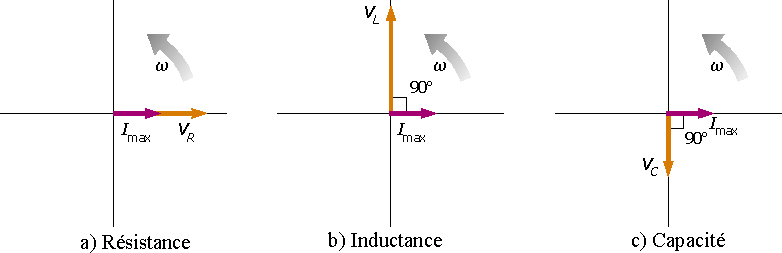
\includegraphics[width=.9\textwidth]{rlc_phaseur.pdf}
    \caption{Tension en fonction du temps à la sortie d'une source de tension alternative.}
    \label{fig:rlc_phaseurs}
  \end{center}
\end{figure}

La longueur du vecteur somme obtenue est alors dénotée $V_{\mathrm{max}}$ et celui-ci fait un angle $\varphi$ par rapport à $I_{\mathrm{max}}$. Comme les tensions $V_L$ et $ V_C$ sont dans des directions opposées et toutes deux perpendiculaires à $V_R$. Nous pouvons alors créer un triangle rectangle et en déduire la grandeur de $\Delta V_{\mathrm{max}}$. Cela s'obtient directement de la manière suivante
\begin{align*}
 V_{\mathrm{max} }&=\sqrt{V_R^2+\left(V_L-\Delta V_C\right)^2}=\sqrt{\left(I_{\mathrm{max} } R\right)^2+\left(I_{\mathrm{max} } X_L-I_{\mathrm{max} } X_C\right)^2} \\
 V_{\mathrm{max} }&=I_{\mathrm{max} } \times \sqrt{R^2+\left(X_L-X_C\right)^2}
\end{align*}
Ceci nous permet par la suite d'exprimer le courant maximal comme
\begin{align*}
    I_{\mathrm{max} }=\frac{V_{\mathrm{max} }}{\sqrt{R^2+\left(X_L-X_C\right)^2}}
\end{align*}

\begin{figure}[H]
  \begin{center}
    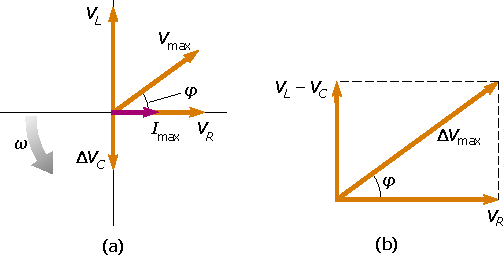
\includegraphics[width=.9\textwidth]{rlc_total.pdf}
    \caption{Tension en fonction du temps à la sortie d'une source de tension alternative.}
    \label{fig:rlc_total}
  \end{center}
\end{figure}

\begin{wrapfigure}{r}{0.4\textwidth}
  \begin{center}
    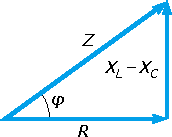
\includegraphics[width=0.27\textwidth]{rlc_triangle.pdf}
    \caption{Représentation de l'impédance d'un circuit.}
    \label{fig:rlc_triangle}
  \end{center}
\end{wrapfigure}

En définissant l'\textbf{impédance} $Z$ du circuit comme
\begin{align*}
    Z\equiv\sqrt{R^2+(X_L-X_C)^2}
\end{align*}
nous retrouvons l'équivalent de la loi d'Ohm, mais dans le cas d'un circuit AC,
\begin{align*}
    V_{\mathrm{max}}(t) = I_{\mathrm{max}}(t)\times Z
\end{align*}
Dans un circuit AC, l'impédance et, donc, le courant, dépend de la résistance, de l'inductance de la capacité et aussi de la fréquence\footnote{Puisque les réactances sont fonctions de la fréquence.}.\\

En retirant le terme $I_{\mathrm{max}}(t)$ de chacun des phaseurs sur la Figure \ref{fig:rlc_total}, il est possible d'obtenir le \textbf{triangle d'impédance} illustré à la Figure \ref{fig:rlc_triangle}. Ce nouveau diagramme de phaseurs nous renseigne directement sur la phase $\phi$ entre le courant et la tension
\begin{align*}
    \varphi=\tan ^{-1}\left(\frac{X_L-X_C}{R}\right)  
\end{align*}

La Figure \ref{fig:rlc_triangle} nous montre que $\cos \varphi = R/Z$ Lorsque $X_L>X_C$ (ce qui se produit à hautes fréquences), la phase est positive, signifiant que le courant est en retard sur la tension, ce qui peut être observé à la Figure \ref{fig:rlc_total}.  Dans ce cas, nous avons affaire à un circuit \emph{inductif}.\\

À l'inverse lorsque $X_L<X_C$, la phase est négative ce qui sous-entend que le courant est en avance sur la tension. Un tel circuit est appelé un circuit \emph{capacitif}.\\

Finalement, lorsque $X_L = X_C$, la phase est de zéro et le circuit est alors purement \emph{résistif}. Ces différentes situations sont décrites à la Figure \ref{fig:table_rlc}.

\begin{figure}[H]
  \begin{center}
    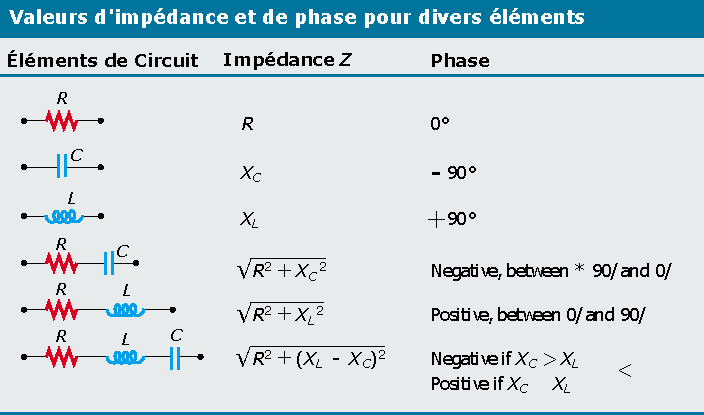
\includegraphics[width=.9\textwidth]{tableau.pdf}
    \caption{Tableau des composante et de leurs effets pour un circuit $RLC$.}
    \label{fig:table_rlc}
  \end{center}
\end{figure}

{\Large \textbf{Le Circuit $\mathrbf{RLC}$}}\\

Commençons tout d'abord par regarder le transport d'énergie dans un circuit RLC comme celui illustré à la Figure \ref{fig:rlc_schema}.\\

Nous pouvons exprimer la puissance totale dissipée comme
\begin{align*}
    P&=I_{\mathrm{max}}\times V_{\mathrm{max}}\\
    &=I_{\mathrm{max}}\sin(\omega t-\phi)V_{\mathrm{max}}\sin \omega t\\
    &=I_{\mathrm{max}}V_{\mathrm{max}}\sin\omega t \sin (\omega t - \varphi)
\end{align*}

Nous pouvons réécrire ceci en utilisant l'identité $\sin (\omega t-\varphi)=\sin \omega t \cos \varphi-\cos \omega t \sin \varphi$ et ainsi obtenir
\begin{equation*}
    P=I_{\mathrm{max} } V_{\mathrm{max} } \sin ^2 \omega t \cos \varphi-I_{\mathrm{max} }V_{\mathrm{max} } \sin \omega t \cos \omega t \sin \varphi
\end{equation*}
Notons que $I_{\mathrm{max}}$, $V_{\mathrm{max}}$, $\varphi$ et $\omega$ sont toutes des constantes. Prenons la moyenne temporelle de l'équation précédente sur plusieurs cycles.\\

Comme démontré plus haut, la moyenne de $\sin ^2 \omega t$ est égale à $\frac{1}{2}$.  De plus, la moyenne du second terme est nulle puisque $\sin \omega t \cos \omega t = \frac{1}{2}\sin 2\omega t$ et que la moyenne d'une fonction sinusoïdale est de zéro. Ainsi, nous pouvons écrire la puissance moyenne dans le circuit comme
\begin{align*}
    P=\frac{1}{2}I_{\mathrm{max}}\times V_{\mathrm{max}}\times\cos\varphi
\end{align*}
Nous pouvons réécrire ceci en fonction des valeurs rms trouvées plus haut comme
\begin{align}
    P=I_{\mathrm{rms}}\times V_{\mathrm{rms}}\times \cos \varphi
    \label{eq:p_phase}
\end{align}
Après quelques simplifications triviales, nous obtenons finalement
\begin{align*}
    P=I_{\mathrm{rms}}^2\times R
    \label{eq:dissipation}
\end{align*}
En d'autres mots, \textbf{la puissance moyenne poussée par la source de tension est convertie en énergie dans la résistance. De plus, seule la résistance agit comme source de dissipation d'énergie dans un circuit.}\\

Nous constatons qu'aucune perte de puissance n'est associée aux condensateurs purs et aux bobines pures dans un circuit AC. Pour comprendre pourquoi cela est vrai, analysons d'abord la puissance dans un circuit AC contenant seulement une source et un condensateur. Lorsque le courant commence à augmenter dans une direction dans un circuit AC, la charge commence à s'accumuler sur le condensateur et une tension apparaît à travers lui. Lorsque cette tension atteint sa valeur maximale, l'énergie stockée dans le condensateur est de $\frac{1}{2}C\times V_{\mathrm{max}}^2$. Cependant, ce stockage d'énergie est seulement momentané. Le condensateur est chargé et déchargé deux fois pendant chaque cycle : la charge est fournie au condensateur pendant deux quarts de cycle et est retournée à la source de tension pendant les deux quarts restants. Par conséquent, la puissance moyenne fournie par la source est nulle. En d'autres termes, aucune perte de puissance ne se produit dans un condensateur dans un circuit AC.\\

Considérons maintenant le cas d'une bobine. Lorsque le courant atteint sa valeur maximale, l'énergie stockée dans la bobine est maximale et est donnée par $\frac{1}{2}LI^2_{\mathrm{max}}$. Lorsque le courant commence à diminuer dans le circuit, cette énergie stockée est renvoyée à la source car la bobine tente de maintenir le courant dans le circuit.\\

L'équation \ref{eq:p_phase} montre que la puissance poussée par une source AC dans n'importe quel circuit ne dépend que de la phase, c'est un résultat qui a de nombreuses applications. Par exemple, lors de la conception de moteurs, machines, générateurs et transformateurs (des appareils qui possèdent une grande charge inductive), des ingénieurs vont souvent introduire des éléments capacitifs dans les circuits d'alimentation pour faire tourner la phase et donc réduire la puissance requise par les appareils.\\
\newpage

{\Large \textbf{Résonnance dans un  circuit $\mathrbf{RLC}$}}\\

Un circuit \emph{RLC} en série est dit en \textbf{résonnance} lorsque le courant qui y circule est maximal.  De façon générale, le courant peut s'écrire
\begin{align*}
    I_{\mathrm{rms}}&=\frac{\Delta V_{\mathrm{rms}}}{Z}\\
    I_{\mathrm{rms}}&=\frac{\Delta V_{\mathrm{rms}}}{\sqrt{R^2+\left(X_L-X_C\right)^2}}
\end{align*}
Comme l'impédance $Z$ dépend de la fréquence de la source, le courrant dans le circuits \emph{RLC} en dépend aussi.  La fréquence $\omega_0$ pour laquelle $X_L-X_C=0$ est appelée la \textbf{fréquence de résonance} du circuit.  Pour trouver $\omega_0$, il faut utiliser la condition
\begin{align*}
    X_L&=X_C\\
    \omega_0 L &= \frac{1}{\omega_0C}\\
    \omega_0 &= \frac{1}{\sqrt{LC}}
\end{align*}
Cette fréquence $\omega_0$ correspond donc à la fréquence naturelle d'oscillation d'un circuit \emph{LC}. À cette fréquence, le courant est aussi en phase avec la tension. À partir de ceci, il est possible de calculer la puissance moyenne en fonction de la féquence. En combinant certaines des équations précédentes, nous en arrivons à 

\begin{align*}
    \langle P \rangle=I_{\mathrm{\mathrm{rms}}}^2 R=\frac{\left(\Delta V_{\mathrm{\mathrm{rms}}}\right)^2}{Z^2} R=\frac{\left(\Delta V_{\mathrm{\mathrm{rms}}}\right)^2 R}{R^2+\left(X_L-X_C\right)^2}
\end{align*}
et puisque $X_L = \omega L$, $X_C = 1/\omega C$ et $\omega_0^2 = 1/LC$, nous pouvons écrire le temps $(X_L-X_C)^2$ comme
\begin{align*}
    (X_L-X_C)^2 = \Bigg{(}\omega  L - \frac{1}{\omega C}\Bigg{)}^2=\frac{L^2}{\omega^2}(\omega^2-\omega_0^2)^2
\end{align*}
En combinant ces deux dernières équations, nous obtenons
\begin{align}
    \langle P \rangle = \frac{(\Delta V_{\mathrm{rms}})^2R\omega^2}{R^2\omega^2+L^2(\omega^2-\omega_0^2)^2}
    \label{eq:puissance}
\end{align}

Cette expression nous montre que \textbf{lorsque} $\omega = \omega_0$\textbf{, la puissance moyenne atteint un maximum et possède une valeur $(\Delta V_{\mathrm{rms}})^2/R$.}  Ce comportement est illustré à la Figure \ref{fig:resonance}. Lorsque la valeur de $R$ diminue, la courbe devient de plus en plus piquée autour de 

\begin{figure}[H]
  \begin{center}
    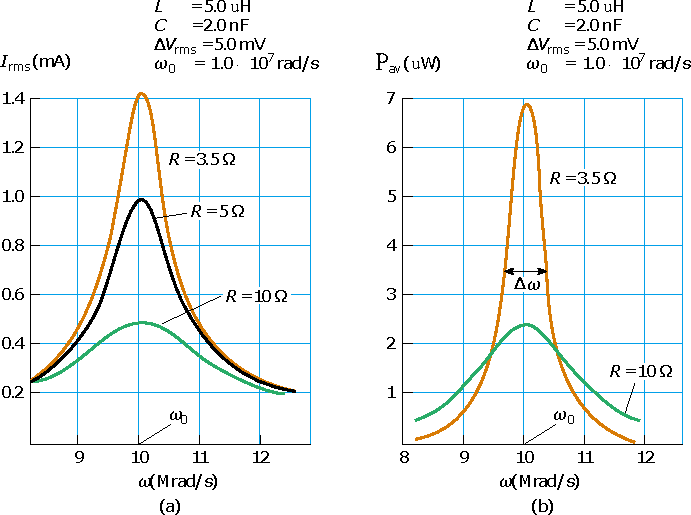
\includegraphics[width=.9\textwidth]{resonances_pics.pdf}
    \caption{Illustration montrant le comportement d'un circuit aux alentours de sa fréquence de résonnance, autant pour le courant que pour la puissance.}
    \label{fig:resonance}
  \end{center}
\end{figure}


$\omega_0$.  Ceci se traduit par un paramètre sans dimension nommé le \textbf{facteur de qualité}, noté $Q$ et qui correspond à 
\begin{align}
    Q=\frac{\omega_0}{\Delta \omega}
    \label{eq:quality}
\end{align}



avec $\Delta \omega$ la largeur correspondant à l'intervalle de fréquences pour lesquelles $\langle P \rangle$ est à la moitié de sa valeur maximale.  $\Delta \omega$ est appelée à largeur à mi-hauteur.  Il est possible de démontrer que $\Delta \omega = R/L$ et, donc, par conséquent, que
\begin{align*}
    Q = \frac{\omega_0 L}{R}
\end{align*}

Tel qu'illustré à la Figure \ref{fig:qualite}, un circuit avec un grand facteur de qualité ne répond qu'à une toute petite gamme de fréquence, tandis qu'un circuit avec un faible facteur de qualité peut détecteur une plus grande plage de fréquences.  De manière typique, dans l'électronique, la valeur de $Q$ varie sur la plage $10^1<Q<10^2$.\\

Un exemple particulier d'un circuit résonnant est une radio.  Un auditeur peut sélectionner une chaîne particulière en variant la valeur d'une capacité, ce qui change la fréquence de

\begin{wrapfigure}{l}{0.4\textwidth}
  \begin{center}
    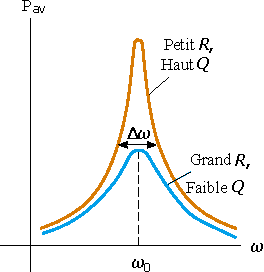
\includegraphics[width=0.4\textwidth]{qualite.pdf}
    \caption{Deux circuits possédant la même fréquence de résonnance peuvent réagir différement à certaines fréquences d'exitation si leur facteurs de qualité diffèrent.}
    \label{fig:qualite}
  \end{center}
\end{wrapfigure}


résonnance du circuit.  Lorsque la résonnance correspond à la fréquence du signal radio entrant émis par la station, le courant dans le circuit augmente.  Le signal reçu est alors envoyé vers les haut-parleurs qui, à leur tour, transforment le signal électrique en signal sonore.  


\end{document}

% Pourquoi ajoute-t-on une résistance au crossover?
% Démontrez la forme pour Q (Problème 72)


